\section{Columnar database}

A columnar database stores data in columns rather than rows. 
This approach is optimized for Online Analytical Processing and data mining tasks, where efficient read operations over large datasets are essential.

In row-oriented databases, modifying a record is straightforward, but querying might involve reading unnecessary data. 
Columnar databases, however, allow for reading only the relevant columns. 
However, writing entire tuples requires multiple column accesses, making columnar databases more suitable for scenarios with high read and lower write demands.
\begin{table}[H]
    \centering
    \begin{tabular}{|l|l|}
    \hline
    \textbf{Advantages}                 & \textbf{Disadvantages}                   \\ \hline
    Data compression                    & Increased disk seek time                 \\ \hline
    Improved bandwidth utilization      & Increased cost of inserts                \\ \hline
    Improved code pipelining            & Increased tuple reconstruction costs     \\ \hline
    Improved cache locality             &                                          \\ \hline
    \end{tabular}
\end{table}
\noindent When tuples need to be analyzed, they are often reconstructed using a large prefetch, which helps minimize the effect of disk seeks across columns.

\paragraph*{Compression}
Columnar databases leverage compression techniques more effectively than row-based databases. 
These databases take advantage of higher data value locality in columns, enabling advanced techniques like run-length encoding.
Additional space can be used to store multiple copies of data in different sort orders, further optimizing query performance.

\subsection{Cassandra}
Originally developed by Facebook and now maintained by the Apache Foundation, Cassandra is a popular column-oriented, NoSQL database widely used for high-throughput applications. 

\subsubsection{Architecture}
Cassandra's architecture is optimized for high availability, scalability, and write-intensive workloads, making it ideal for distributed, flexible data storage systems. 
Its column-oriented design, combined with a masterless structure, eliminates single points of failure while providing tunable consistency for varying application requirements.

Cassandra's masterless architecture ensures no single node holds ultimate control, distributing data across a ring of nodes. 
This ring topology connects servers in a circular fashion, enabling redundancy and fault tolerance.
Each node in the ring is responsible for a portion of the data, and data placement follows a clockwise strategy to the next nodes in the ring, ensuring even distribution.
\begin{figure}[H]
    \centering
    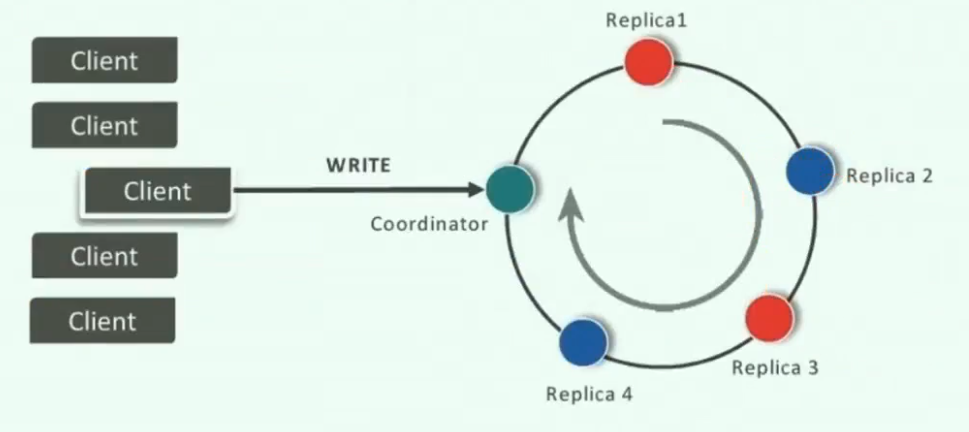
\includegraphics[width=0.65\linewidth]{images/ring.png}
    \caption{Ring architecture}
\end{figure}

Cassandra minimizes network overhead, except during rare gossip storms. 
Nodes periodically exchange small membership updates via the gossip protocol, ensuring consistent and accurate cluster state awareness.
Each node gossips with up to three peers, fostering rapid convergence and anti-entropy to synchronize data efficiently.

\paragraph*{Gossip protocol}
Cassandra uses a lightweight gossip protocol to maintain cluster state while minimizing bandwidth consumption. 
Each node communicates with a small subset of peers (up to three) during a gossip round. 
This exchange helps disseminate cluster information efficiently and introduces a layer of anti-entropy, allowing data to converge more quickly across the cluster. 
Nodes periodically share their membership list, updating their local view upon receiving updates from peers. 
This ensures the cluster remains synchronized and resilient, even in the face of failures or network issues.

The operations that we can do are: 
\begin{itemize}
    \item \textit{Write}: Cassandra prioritizes speed and availability for writes, avoiding disk seeks and locks to maintain scalability.
    When a client sends a write request, it is directed to a coordinator node, which identifies responsible replicas and forwards the data. 
        If a replica is temporarily unavailable, the coordinator buffers the data, ensuring eventual consistency via a mechanism called hinted handoff.
        Data is initially written to a commit log for durability, then updated in an in-memory structure called the memtable. 
        Over time, the memtable is flushed to disk as SSTables, which are indexed and include bloom filters for efficient reads. 
        Periodic compaction merges updates and applies tombstones to optimize storage.
    
        A bloom filter is a compact and efficient data structure used to represent a set of items. 
        It allows quick membership checks to determine if an item is possibly in the set, with minimal memory overhead.
        While bloom filters can produce false positives they never produce false negatives, ensuring that if an item is in the set, it is always identified as such. 
        This makes bloom filters highly effective for applications where occasional false positives are acceptable, but false negatives are not.
    \item \textit{Delete}: deletions are handled lazily by adding a tombstone marker rather than immediately removing the data. 
        These tombstones are processed during compaction to permanently delete the marked records, reducing overhead and improving write performance.
    \item \textit{Read}: reads often involve querying the closest replica for data, but the coordinator may contact multiple replicas to ensure consistency. 
        If discrepancies arise between replicas, the system initiates a background process called read repair to synchronize the data. 
        While reads may be slower than writes due to consistency checks, they remain efficient through the use of memtables, commit logs, and bloom filters to limit disk access.
\end{itemize}

\paragraph*{Consistency levels}
Cassandra provides flexible consistency levels, allowing clients to choose based on application needs:
\begin{itemize}
    \item \texttt{ANY}: data can be written to any node (even non-replicas).
    \item \texttt{ONE}: at least one replica must confirm.
    \item \texttt{QUORUM}: a majority of replicas (across all datacenters) must confirm.
    \item \texttt{LOCAL\_QUORUM}: majority confirmation in the coordinator's datacenter.
    \item \texttt{EACH\_QUORUM}: majority confirmation in each datacenter.
    \item \texttt{ALL}: all replicas in all datacenters must confirm.
\end{itemize}

\subsubsection{Data model}
In Cassandra, data is organized into column families, which are analogous to tables in SQL but are more flexible and can have unstructured, client-specified schemas. 
Column families allow the storage of sparse data, where some columns may be missing in specific rows, fitting Cassandra's NoSQL model.

Each Cassandra keyspace functions similarly to a database, typically used per application with certain configurations set per keyspace. 
The primary elements in Cassandra's data model include:
\begin{enumerate}
    \item \textit{Keyspace}: equivalent to a database, typically unique per application.
    \item \textit{Column family}: groups records of similar types, stored as sparse tables.
    \item \textit{Columns}: each column has three parts:
        \begin{itemize}
            \item \textit{Name}: a byte array used for sorting, querying, and indexing.
            \item \textit{Value}: a byte array; typically not queried directly.
            \item \textit{Timestamp}: used for conflict resolution, with the most recent write winning.
        \end{itemize}
\end{enumerate}
Additionally, Cassandra supports super columns, which group columns under a common name but lack indexing for sub-columns. These are often used to denormalize data from standard column families.
\begin{figure}[H]
    \centering
    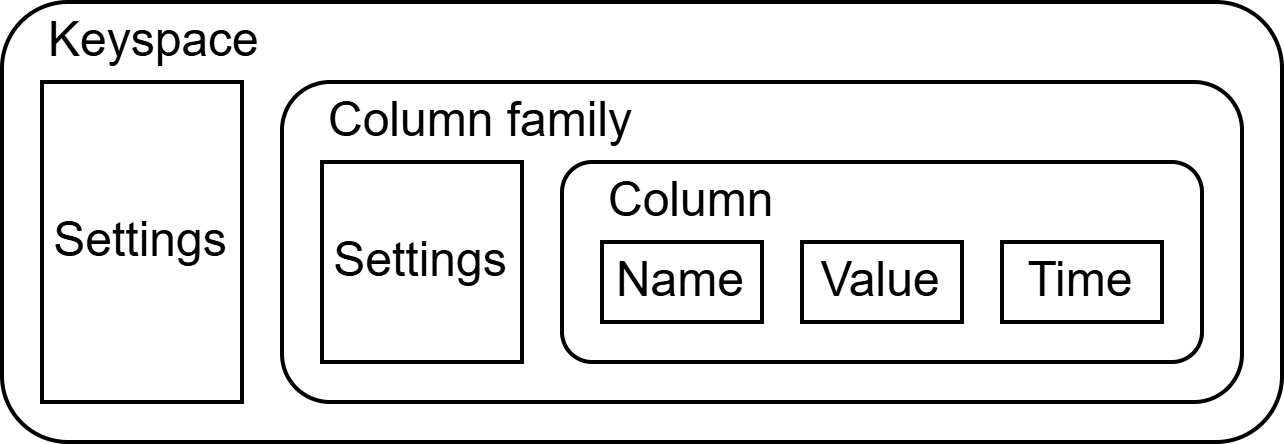
\includegraphics[width=0.75\linewidth]{images/cas.png}
    \caption{Cassandra data model}
\end{figure}

\subsubsection{Query language}
To interact with Cassandra, developers can use the API for various read and write operations:
\begin{lstlisting}[style=Java]
// retrieve a specific column at the given path
get(): Column
// retrieve a set of columns in one row specified by the slice predicate
get_slice(): List<Column>
// retrieve slices for multiple keys based on a SlicePredicate
multiget_slice(): Map<key, List<Column>>
// retrieve multiple columns according to a specified range
get_range_slices(): List<KeySlice>
\end{lstlisting}
For writing operations, Cassandra provides commands such as:
\begin{lstlisting}[style=Java]
// insert a new element in a column
client.insert()
// update an existing element in a column
batch_mutate()
// remove an existing element from a column
remove()
\end{lstlisting}

\paragraph*{CQL}
Cassandra also supports SQL since it is based in tables with a single column.
The main difference is that in relational databases we have a domain-based model, while in columnar databases we have a query-based model. 
Thus, in this case we start from the queries, and then we design the data model based on that since each column has a key that is used to filter all the elements in the column. 

Rows are distributed across the cluster based on the partitioning strategy:
\begin{itemize}
    \item \textit{Random partitioning}: uses the hash of the row key for uniform data distribution.
    \item \textit{Order-preserving partitioning}: uses the actual row key to maintain a natural order.
\end{itemize}
\noindent To create a keyspace, use the following command:
\begin{lstlisting}[style=CQL]
CREATE KEYSPACE identifier 
WITH properties
\end{lstlisting}
A table can have multiple clustering and partition keys. 
The first set of values is called the partition key, and it determines how the data is distributed across the Cassandra nodes. 
The second set of values is the clustering key, which defines how the data is stored within each partition, specifically the sorting order.
\begin{lstlisting}[style=CQL]
PRIMARY KEY ((partition_key, ...), clustering_key, ...)
\end{lstlisting}
When creating a table, you can use Clustering Keys to specify the order in which data is stored.
\begin{lstlisting}[style=CQL]
CREATE TABLE table_name (column_name column_type, ...) 
WITH CLUSTERING ORDER BY (key ASC, ...)
\end{lstlisting}
To verify whether a keyspace or table has been successfully created, you can use the \texttt{describe} command. 
t can also be applied to check other elements:
\begin{lstlisting}[style=CQL]
DESCRIBE keyspaces
\end{lstlisting}
Before performing operations on tables, you need to specify the keyspace you're working with:
\begin{lstlisting}[style=CQL]
USE keyspace_name
\end{lstlisting}
Indexes are crucial in Cassandra tables as they allow for efficient querying of columns. 
While this advantage might not be obvious with small datasets, it becomes essential when dealing with larger datasets.
To create a secondary index, use the following command:
\begin{lstlisting}[style=CQL]
CREATE INDEX identifier
ON table_name(column_name)
\end{lstlisting}